\chapter{Desarrollo del Sistema Propuesto}
En este capítulo se desarrolla la solución al problema de la falta de validacion de documentos digitales emitidos por la Secretaría 
de Extensión de la \gls{fce} de la \gls{unam}.
Se realiza el diseño teórico que se pretende aplicar y se define su funcionamiento y las relaciones entre las
herramientas y tecnologías en la implementación. 

\section{Tecnologías y Herramientas Seleccionadas}
Las tecnologías y herramientas seleccionadas para el desarrollo de la propuesta son:
\begin{enumerate}
    \item La red de prueba llamada Ropsten, esta  Blockchain de prueba  permite publicar los smart contract
    y la emisión de su token de prueba es de forma gratuita, cuenta con pocos nodos pero el objetivo 
    de su uso es hacer pruebas en esta red, su comportamiento es similar a otra  Blockchain con maquina virtual de Ethereum \cite[]{dannen_introducing_2017}.
    \item Solidity como lenguaje de programación para los contratos inteligentes \cite[]{dannen_introducing_2017,bragagnolo_smartinspect_2018}.
    \item Node JS con su gestor de paquetes para instalar las librerías necesarias.
    \item Web3.js una librería de javascript que permite conectarse a la  Blockchain de una manera más rápida y abstrayendo la complejidad de la comunicación
    con la Blockchain \cite[]{dannen_introducing_2017}.
    \item SHA-256 un algoritmo de hash, pero también existen diferentes  librerías de  javascript que permite generar un hash a partir de caracteres.
    \item Vue.js un framework de javascript, para facilitar el desarrollo del front-end, reutilizando partes de otros proyectos open sources.\cite[]{vuejs_introduction_nodate}
    \item Para la publicación de los contratos inteligente se usará Remix, es una de las tecnologías ya mencionadas y su uso 
    es intuitivo \cite[]{remix_deploy_nodate}.

\end{enumerate}

Estas tecnologías permitirán crear el sistema para validar los documentos de la Secretaría de Extensión de la \gls{fce} de la \gls{unam}, dando el beneficio 
a terceros de verificar que el contenido de un documento  es correcto y no fue alterado \cite[]{brys_cadena_2019}. 

\section{Diseño de la Lógica}
A continuación se muestra un diagrama para comprender los datos  esenciales para el diseño del sistema.

\begin{figure}[H]
  \centering
  {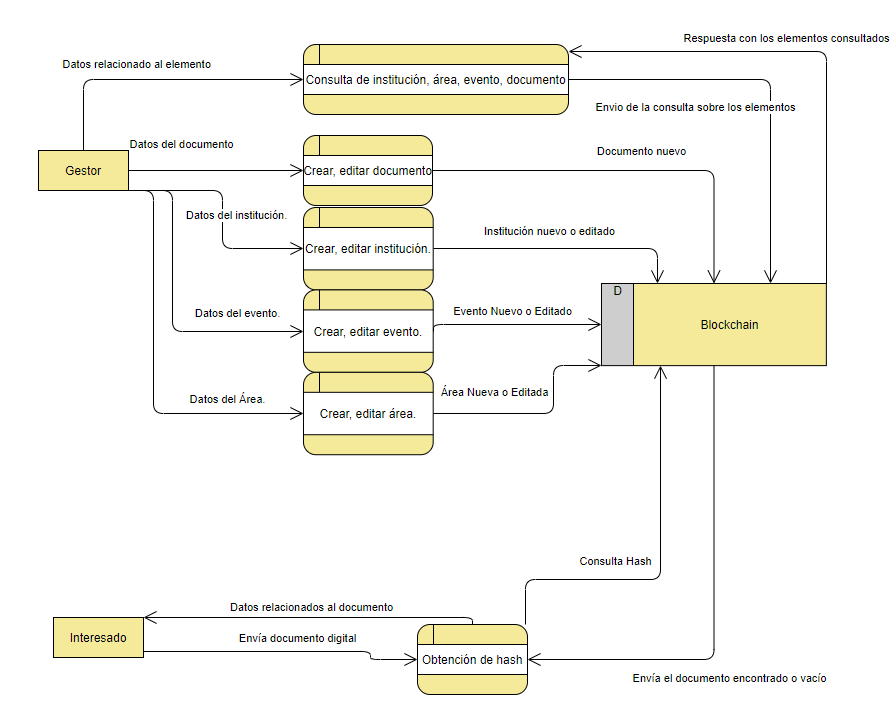
\includegraphics[scale=0.6]{Diagrama_Validacion_Documento.png}}
  \caption{Diagrama de Flujos de datos, Fuente: producción propia.}
  \label{img:flujo-datos}
\end{figure}

En la figura \ref{img:flujo-datos} se observa el flujo de los datos que se manejan en una validación de certificados, principalmente se almacenan los datos en la Blockchain y son leidos por las personas interesadas. Los responsables 
de sus áreas deben  almacenar los datos en la Blockchain, esto permitirá validar que los documentos almacenadas solamente
serán cargados por personal autorizado.    

% El flujo de los datos de la figura \ref{img:flujo-datos} será principalmente almacenar los datos relacionados a un documento digital específico. Por parte de 
% uno o algunos responsables, ya que si cualquier individuo puede almacenar esta información, no tendría ninguna validez,
% por lo tanto solo los documentos almacenados mediante el uso del smart contract  serán válidos.

Los interesados en el diagrama representan a cualquier individuo (como el propio dueño del documento digital, o una autoridad de la organización o persona externa de ella), 
se puede obtener datos relacionados con el documento quién fue el emisor o si el documento fue realmente subido por la organización. 
Pero para poder realizar tal verificación debe tener el documento digital en su posesión; de esta forma comprobar si 
el contenido del documento no fue modificado y que fue emitido por la organización.

Los gestores son los encargados de almacenar la información y serían las personas responsables 
de los documentos emitidos.

\section{Diseño de Sistema}\label{s:system_design}

En la sección \ref{ss:basesistema}  se explica de manera genérica, los datos necesarios 
para validar un documento digital en base a los estándares BlockCert y OpenCert.
Para ello se diseña un diagrama de la figura \ref{img:diagrama_clases} para la propuesta del sistema para validación de documentos:  

\begin{figure}[H]
    \centering
    {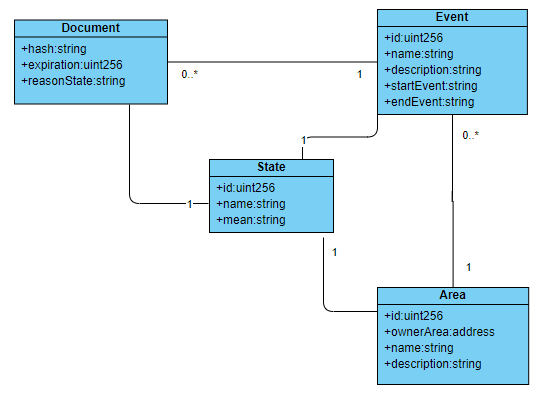
\includegraphics[scale=0.7]{diagrama_clases.png}}
    \caption{Diagrama de domino, Fuente: producción propia.}
    \label{img:diagrama_clases}
  \end{figure}

  En la figura \ref{img:diagrama_clases} se puede observar la propuesta de  construcción del sistema basándose 
  en el estándar de BlockCerts donde se almacenan los hashes del documento e información relacionada a ella \cite[]{blockcerts_introduction_nodate,criptomonedas_tv_entrevista_2018,blockcerts_faq_nodate}, 
  el diagrama muestra un área que es la responsable 
  de emitir los certificados, sin revelar datos de personas o contenido del documento. Por lo tanto el objetivo
  de no incluir  datos sensibles quedan cubiertos. 

  Se analizaron los requerimientos de la universidad y en conjunto a la entrevista (A.L., comunicación personal, 02/10/2020) para poder diseñar la lógica del sistema. Se incluyeron administradores o los propietarios (owner) 
  de las áreas, serían los responsables de almacenar los hashes de  documentos que se generen en los Eventos de las Áreas,
  cuando se habla de los eventos, se los trata como  genéricos, un evento puede ser una clase, una charla, un congreso o inclusive
  una determinada hora del día, de esta manera los documentos pueden estar relacionados a los eventos que ocurren.

  La construcción, el almacenamiento  y lectura  de datos de una aplicación  en la  Blockchain es diferente a una 
  aplicación centralizada, por ejemplo, los datos almacenados no se consultan mediante lenguaje SQL, tampoco se puede agregar nuevas
  variables una vez almacenado en la Blockchain, en cambio en una base de datos centralizada si se pueden agregar nuevos atributos \cite[]{dannen_introducing_2017,mayor_Blockchain_2017}.

 En resumen el dominio comprende áreas, eventos, estados y los documentos cada uno de ellos
 almacena datos representativos y básicos para validar la existencia de un documento digital en la Blockchain. 

  \subsection{Estructura del Smart Contract}
  Definir  los datos necesarios para la propuesta del sistema, permite dar forma a 
  la estructura del smart contract, ya que éste no cambiará una vez que sea publicado en la Blockchain, pero no significa
  que se pueda publicar otras versiones. La propuesta es utilizar una  Blockchain de prueba  para realizar todos los intentos necesarios 
  hasta obtener el funcionamiento del sistema. 

  La estructura del smart contract será como se refleja en la figura \ref{img:smart_contract_structure}, a continuación se explican cada parte de ella:

  
\begin{figure}[hbt!]
    \centering
    {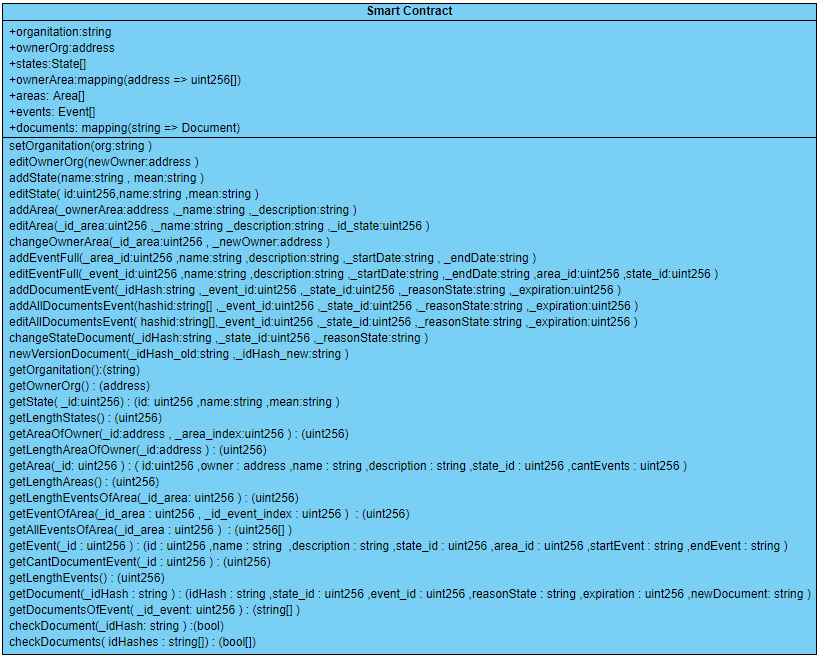
\includegraphics[scale=0.5]{smart_contract_abstract.png}}
    \caption{Smart Contract estructura, Fuente: producción propia.}
    \label{img:smart_contract_structure}
  \end{figure}
Los atributos (de la figura \ref{img:smart_contract_structure} ) que almacenarán los datos necesarios serán los siguientes :
  \begin{itemize}
    \item \textit{\textbf{ organitation: string}}, se almacenará el nombre de la organización responsable de las áreas, eventos y todos los documento digitales.
    \item \textit{\textbf{ownerOrg: address}}, la dirección de la cuenta del único responsable para manejar todos los datos del smart contract.
    \item \textit{\textbf{states: State[]}}, los posibles estados que maneja el sistema, como ser estado revocado, el cual el estándar BlockCert y OpenCert lo usan \cite[]{blockcerts_faq_nodate,opencerts_gestion_nodate}.
    \item \textit{\textbf{ownerArea:mapping(address => uint256[])}}, son el conjunto de direcciones que están encargadas de manejar una o varias áreas especificas. Estos owner deberían ser agregados por el owner de la organización para evitar que un individuo desconocido tenga el poder de modificar datos.
    \item \textit{\textbf{areas: Area[]}}, el conjunto de áreas de la organización.
    \item \textit{\textbf{events: Event[]}}, los eventos que pueden surgir en un área especifica y encargados de generar los documentos digitales.
    \item \textit{\textbf{documents: mapping(string => Document)}}, los hashes de documentos asociado a la información del documento.
    \end{itemize}

    La notación que se utilizó para el diagrama \ref{img:smart_contract_structure} para los tipos de datos son de la misma manera
    en la que se definen en Solidity,
    como por ejemplo la definición de mapping(string => Document). Esto sirve para definir  una variable  que recibe como
    índice un string por ejemplo “A”  referencia un documento almacenado en la Blockchain. El string se creó como índice para 
    que el usuario pueda usar cualquier tipo de algoritmo de hash y el sistema permita almacenar en la  Blockchain sin tomar en cuenta la función hash
   , esta idea es usada por los estándares ya mencionados \cite[]{opencerts_gestion_nodate,blockcerts_introduction_nodate,blockcerts_faq_nodate}. 

    Los métodos para realizar cambios en los datos del sistema:
    \begin{itemize}
      \item \textit{\textbf{setOrganitation(org:string)}}, el método permite cambiar el nombre de la organización, sólo debe ser ejecutado por el propietario de la organización.
      \item \textit{\textbf{editOwnerOrg(newOwner:address)}}, permite cambiar al único usuario que podrá ejecutar todos los métodos.
      \item \textit{\textbf{addState(name:string, mean:string)}}, name es el nombre del estado y mean el significado o para qué se usaría. El método agrega un nuevo estado que podrá ser usado por las áreas, eventos y documentos.
      \item \textit{\textbf{editState( id:uint256, name:string, mean:string)}}, edita el nombre y el significado del estado.
      \item \textit{\textbf{addArea(ownerArea:address, name:string, description:string)}}, crea un nuevo estado y pasa por parámetros la dirección del dueño o responsable del área a crear, el nombre, y una descripción como dato extra. El único que puede ejecutar este método es la dirección que concuerde con la ownerOrg
      \item \textit{\textbf{editArea(id\_area:uint256, name:string description:string, id\_state:uint256)}}, el id que representa el área a editar, los datos a modificar como el nombre, la descripción y el estado actual.
      \item \textit{\textbf{changeOwnerArea(id\_area:uint256, newOwner:address)}}, permite cambiar el propietario de un área específica.
      \item \textit{\textbf{addEventFull(area\_id:uint256, name:string, description:string, startDate:string, endDate:string)}}, agrega un evento a la  Blockchain relacionándolo, con un área especifica.
      \item \textit{\textbf{editEventFull(event\_id:uint256, name:string, description:string, startDate:string, endDate:string, area\_id:uint256, state\_id:uint256)}}, edita la mayoría de los atributos de un evento.
      \item \textit{\textbf{addDocumentEvent(idHash:string, event\_id:uint256, state\_id:uint256, reasonState:string, expiration:uint256)}}, crea un documento nuevo con relación a un evento particular y una fecha de vencimiento para el documento digital. La fecha
      es representada por un valor numérico o \gls{TimeStamp}.
      \item \textit{\textbf{addAllDocumentsEvent(hashid:string[], event\_id:uint256, state\_id:uint256, reasonState:string, expiration:uint256)}}, permite almacenar muchos documentos enviando un array de hashes y 
      los atributos iguales que tendrán los documentos, por ejemplo todos los documentos serán del mismo evento, tendrán el mismo estado  y fecha de vencimiento.
      \item \textit{\textbf{editAllDocumentsEvent(hashid:string[], event\_id:uint256, state\_id:uint256, reasonState:string, expiration:uint256)}}, edita todos los documentos que se encuentran en el array de hashes.
      \item \textit{\textbf{changeStateDocument(idHash:string, state\_id:uint256, reasonState:string)}}, cambia el estado de un solo documento.
      \item \textit{\textbf{newVersionDocument(idHash\_old:string, idHash\_new:string)}}, se le asigna una nueva versión a un documento antiguo, idHash\_old es el documento antiguo o idHash\_new es el hash del nuevo documento,
      esto sirve para mantener versiones de un solo documento. 
    \end{itemize}

    Y por último, los métodos para lectura de los datos son:

    \begin{itemize}
      \item \textit{\textbf{getOrganitation():(string)}}, retorna un string que es el nombre de la organización.
      \item \textit{\textbf{getOwnerOrg() : (address)}}, devuelve la dirección del dueño o propietario, el cual podrá ejecutar todos los métodos.
      \item \textit{\textbf{getState( id:uint256) : (id: uint256, name:string, mean:string )}}, retorno los atributos del estado que tenga el id pasado por un parámetro.
      \item \textit{\textbf{getLengthStates() : (uint256)}}, obtiene la cantidad de estados almacenados.
      \item \textit{\textbf{getAreaOfOwner(id:address, area\_index:uint256 ) : (uint256)}}, obtiene el id de un área de un propietario de área.
      \item \textit{\textbf{getLengthAreaOfOwner(id:address ) : (uint256)}}, obtiene la longitud o la cantidad de areas de un propietario de área.
      \item \textit{\textbf{getArea(id: uint256 ) : ( id:uint256,owner : address,name : string,description : string,state\_id : uint256,cantEvents : uint256 )}}, obtiene un área a partir de un id.
      \item \textit{\textbf{getLengthAreas() : (uint256)}}, obtiene la cantidad de áreas que hay almacenado en la Blockchain.
      \item \textit{\textbf{getLengthEventsOfArea(id\_area: uint256) : (uint256)}}, la cantidad de eventos que están relacionado a un área.
      \item \textit{\textbf{getEventOfArea(id\_area : uint256, id\_event\_index : uint256)  : (uint256)}}, obtiene el id un evento relacionado a un área.
      \item \textit{\textbf{getAllEventsOfArea(id\_area : uint256 )  : (uint256[])}}, trae todos los id de eventos de un área.
      \item \textit{\textbf{getEvent(id : uint256) : (id : uint256,name : string ,description : string,state\_id : uint256,area\_id : uint256,startEvent : string,endEvent : string )}}, obtiene los atributos de un evento.
      \item \textit{\textbf{getCantDocumentEvent(id: uint256) : (uint256)}},   la cantidad de documentos relacionado a un evento.
      \item \textit{\textbf{getLengthEvents() : (uint256)}}, cantidad de eventos que existen almacenados.
      \item \textit{\textbf{getDocument(idHash : string) : (idHash : string,state\_id : uint256,event\_id : uint256,reasonState : string,expiration : uint256,newDocument: string )}}, obtiene todo los atributos de un documento a partir de su hash.
      \item \textit{\textbf{getDocumentsOfEvent(id\_event: uint256) : (string[])}}, obtiene todos los hashes de los documentos relacionado a un evento.
      \item \textit{\textbf{checkDocument(idHash: string) :(bool)}}, devuelve true si el hash del documento esta almcenado en la Blockchain.
      \item \textit{\textbf{checkDocuments(idHashes : string[]) : (bool[])}}, a partir de un array de hashes de documentos devuelve en el mismo orden true o false dependiendo si existe o no en la Blockchain
      respectivamente.
    \end{itemize}

    \subsection{Roles y Permisos}
    En la propuesta de sistema se utiliza un smart contract para el código almacenado en la Blockchain. Para ello también es necesario definir los responsables de gestionar los datos.
    Se establecen dos niveles, el primero es un usuario que pueda gestionar todo los datos, como un administrador. 
    Por ende, se debe definir el rol de un usuario o propietario del smart contract, que sea el único que tenga el poder de crear nuevas áreas,
    cambiar en nombre a la organización, editar los datos de las áreas, agregar o quitar responsables de cada área. 
    El otro nivel son los usuarios encargados de una o muchas  áreas, los cuales tienen la responsabilidad de gestionar los documentos y eventos de un área especifica,
    para ello el administrador o el propietario del smart contract decide quiénes son los operarios o encargados de crear los documentos digitales y almacenarlos en la  Blockchain mediante
    su hash.
    Esto es importante para evitar que usuarios externos a la organización controlen los documentos emitidos por la entidad. Para ello se crean los roles o niveles de seguridad.
    También habrá un usuario que no tiene el poder de modificar los datos almacenados, simplemente podrá consultar 
    acerca de los documentos y validaciones, es el individuo que requiere conocer la validez del documento y comprobar que es emitido por la organización. 
    En resumen se definen dos niveles: nivel de administrador es el encargado y responsable de todo los datos almacenados, por otro lado un nivel de encargados de  áreas.
  \subsubsection{Estructura de permisos}
  Todos los usuarios tendrán acceso a leer sus datos, por eso desde el inicio   se evita almacenar datos sensibles relacionados
  a los dueños de los documentos, mientras que los datos de la organización son públicos y pueden ser almacenados. 
  En esta sección se definirán qué comportamiento tendrán los roles y qué permisos según los niveles de usuarios. Al analizar los datos sobre los métodos y las necesidades 
  a satisfacer, se parte de tres niveles: 
  \begin{enumerate}
    \item Nivel público: el usuario podrá consultar datos almacenados, (cómo verificar si un documento existe en la Blockchain).
    \item Nivel de propietario de área: son los encargados de almacenar y crear los eventos relacionado a sus áreas, también de gestionar los documentos digitales, cambiando sus estados,
    agregando nuevas versiones.
    \item Nivel de propietario del smart contract: es la única dirección que tiene permiso de ejecutar todos los métodos. Puede cambiar el nombre de la organización,
    asignar nuevos propietarios de áreas, crear áreas, y hacer lo mismo que los demás niveles. 
  \end{enumerate}
  


\section{Desarrollo del Smart Contract}
A continuación se detallan las herramientas y las manera de utilizarlas para el desarrollo 
del Smart Contract.

\subsection{Instalación de Metamask}

Como primer paso, hay que instalar el plugin de Metamask de la  página web oficial   el navegador que se usará de prueba (en este proceso, es  Google Chrome) 
tal como se muestra en la  figura \ref{img:metamask_install}.
\begin{figure}[H]
  \centering
  {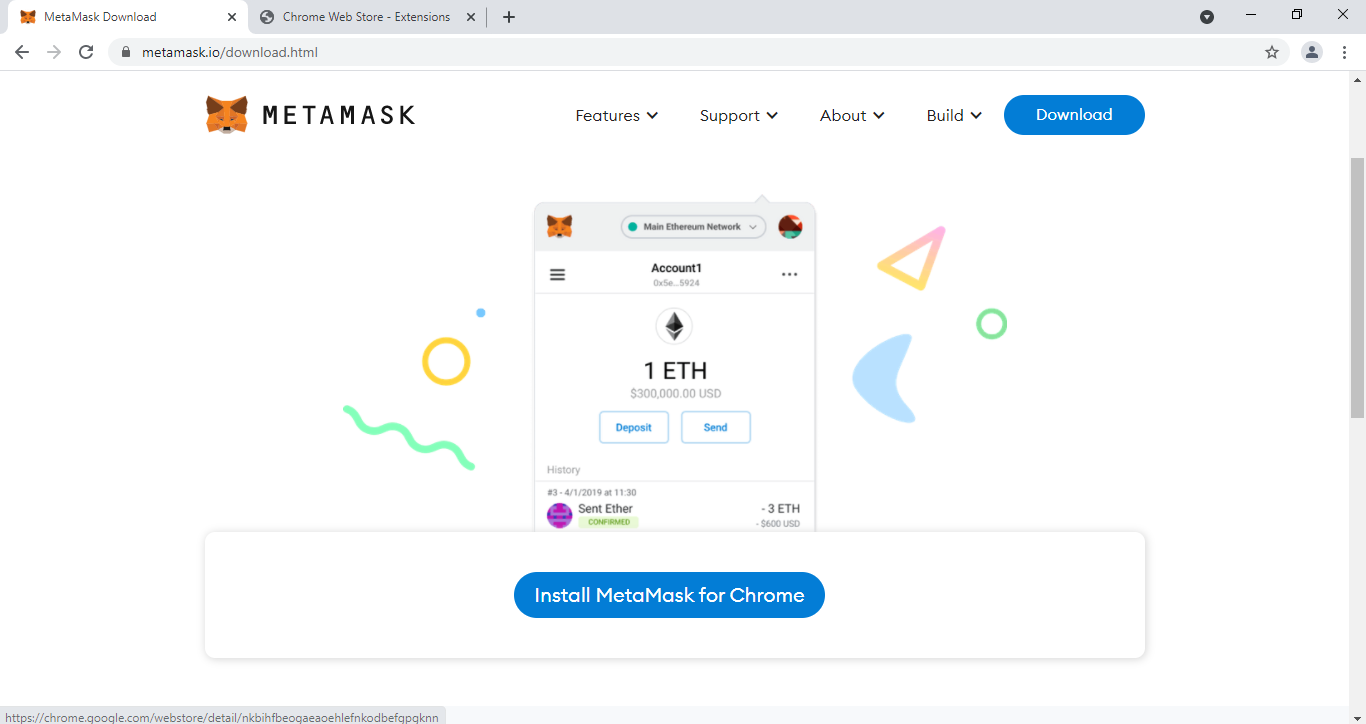
\includegraphics[scale=0.4]{metamask_install.png}}
  \caption{Página para descargar Metamask, Fuente: captura de pantalla.}
  \label{img:metamask_install}
\end{figure}

Se agrega el plugin al navegador como se ve en la figura \ref{img:metamask_add}, luego
se abrirá una nueva pestaña o en caso que no aparezca deberá buscar Metamask en sus extensiones del navegador 
para hacer clic donde este le redirigirá a una nueva pestaña para crear o importar su wallet.
Los pasos son hacer clic en Get Stated visto en la figura \ref{img:metamask_getstarted}.



\begin{figure}[H]
  \centering
  {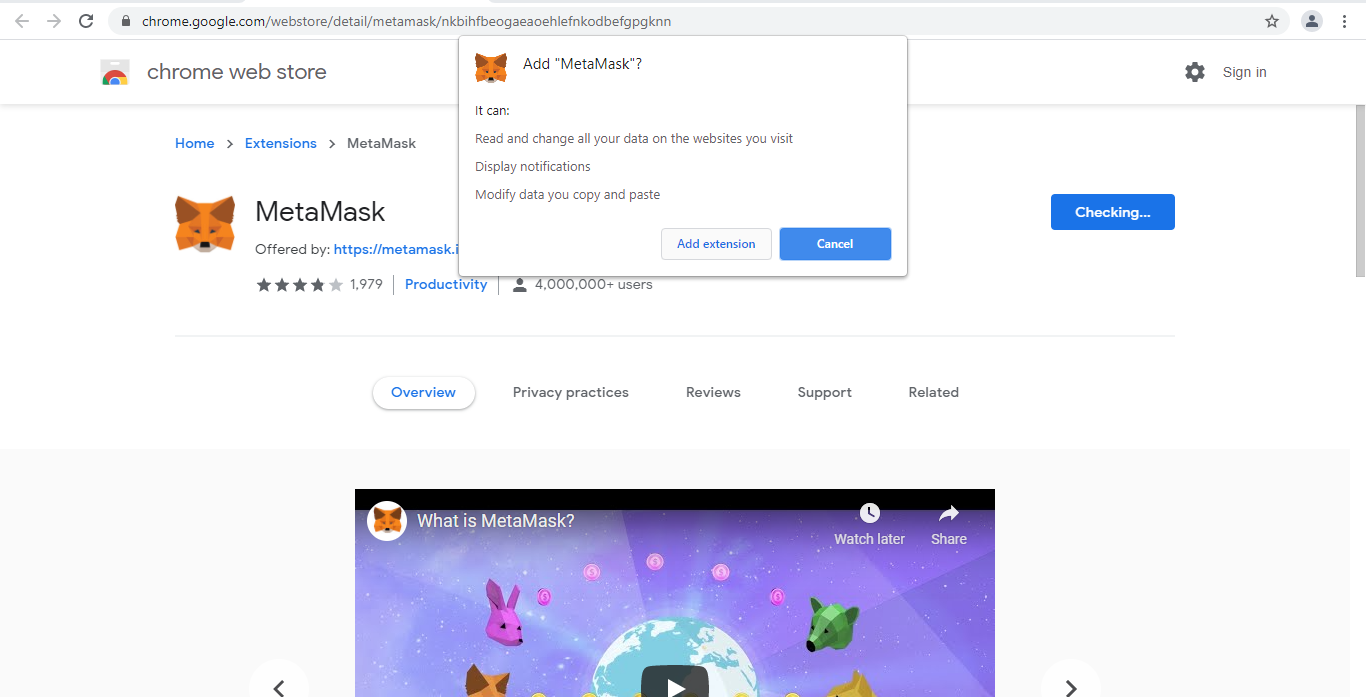
\includegraphics[scale=0.4]{metamask_addplugin.png}}
  \caption{Agregando el plugin, Fuente: captura de pantalla. }
  \label{img:metamask_add}
\end{figure}

\begin{figure}[H]
  \centering
  {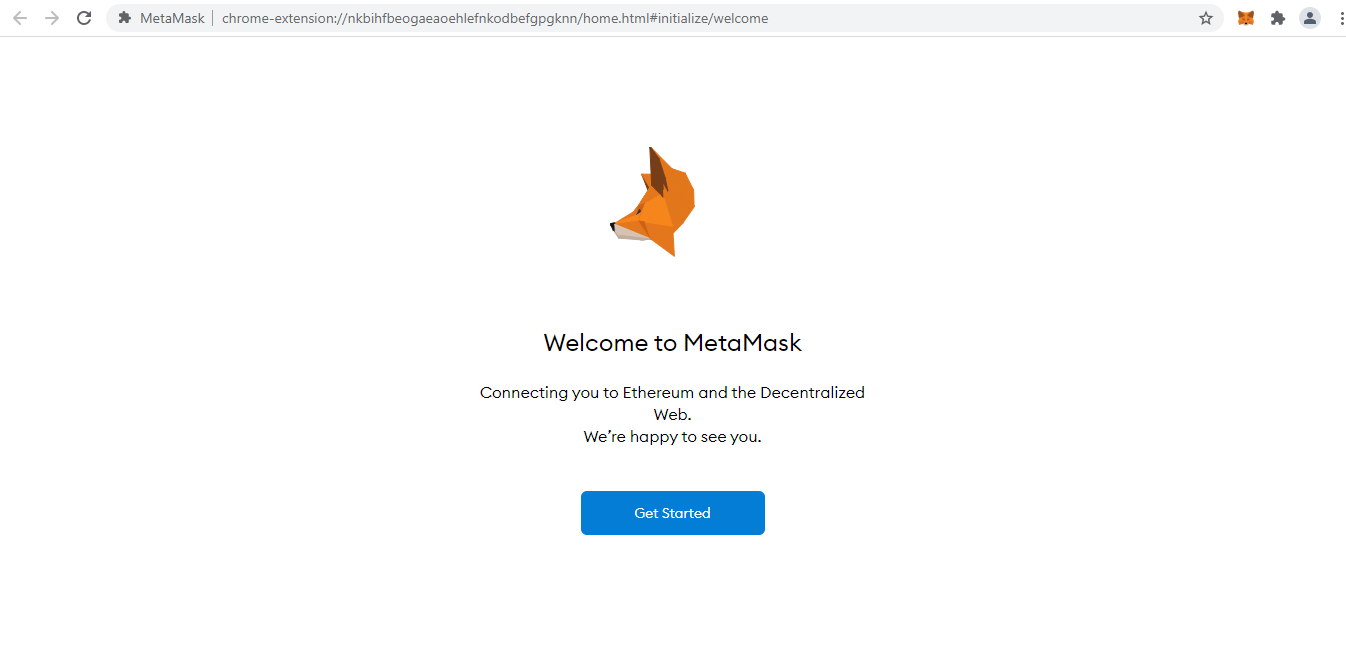
\includegraphics[scale=0.4]{metamask_getstarted.png}}
  \caption{Inicio para crear o importar una wallet, Fuente: captura de pantalla.}
  \label{img:metamask_getstarted}
\end{figure}

Como siguiente paso hay que crear una wallet. Esto es importante para poder interactuar con el sistema
(específicamente con los smart contract). Leer los términos y condiciones si están de acuerdo aceptarlos,
el siguiente paso es crear una contraseña, esta sirve para acceder a Metamask en el computador local, evita que otro usuario pueda acceder si no conoce la contraseña y agrega un nivel más de seguridad, ya que  se pueden realizar diferentes operaciones.

\begin{figure}[H]
  \centering
  {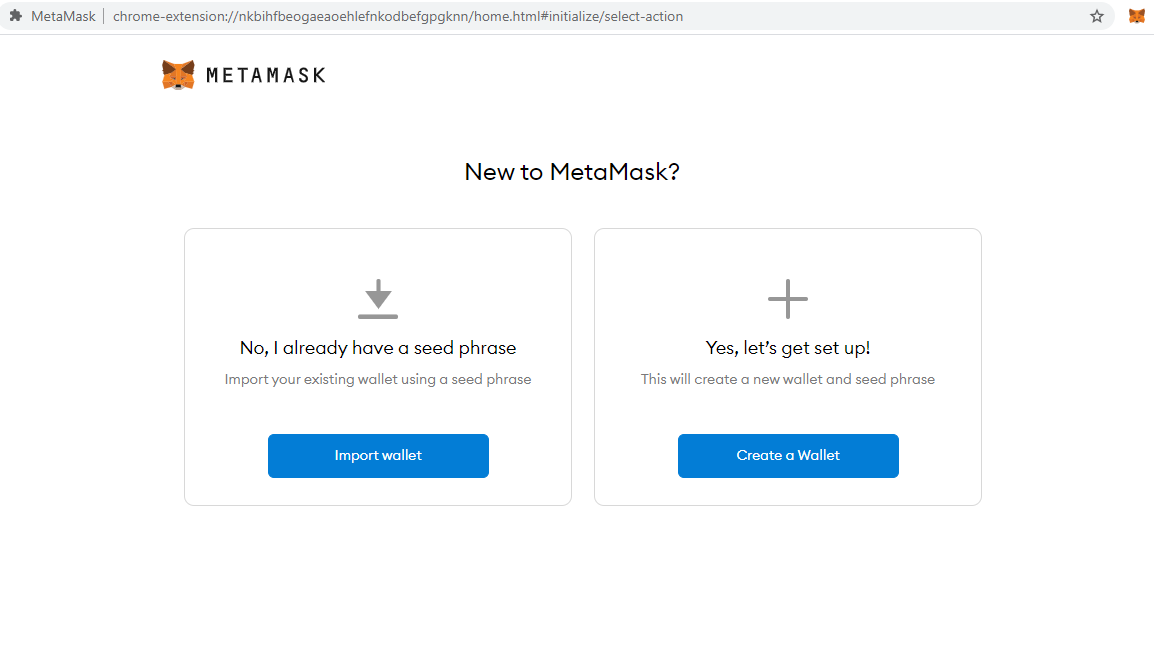
\includegraphics[scale=0.4]{metamask_create.png}}
  \caption{Menú crear wallet,  Fuente: captura de pantalla. }
  \label{img:metamask_create}
\end{figure}

\begin{figure}[H]
  \centering
  {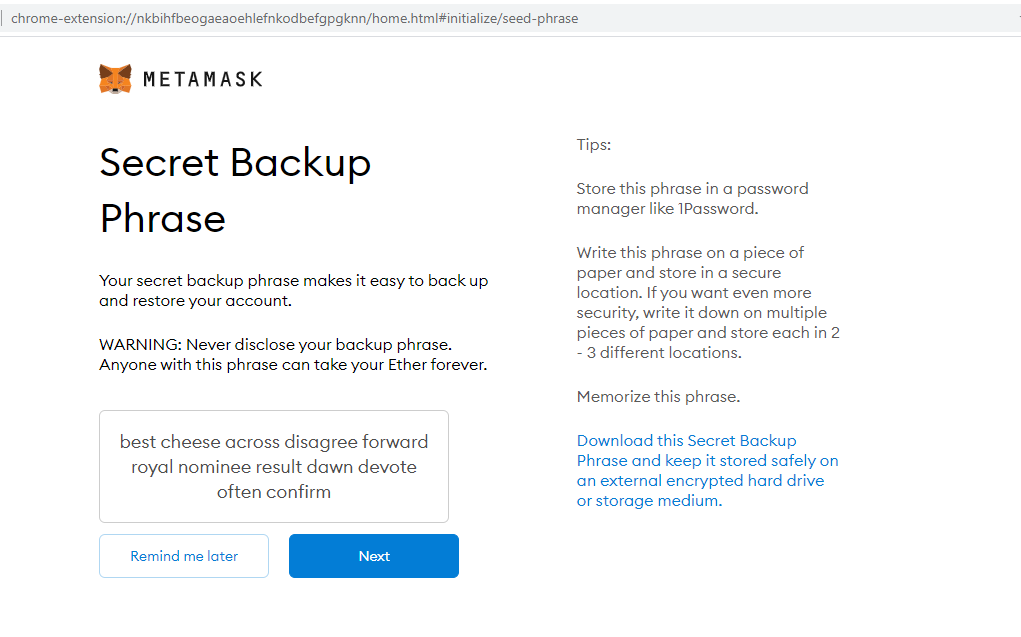
\includegraphics[scale=0.4]{metamask_semilla.png}}
  \caption{Frases semillas,  Fuente: captura de pantalla. }
  \label{img:metamask_semilla}
\end{figure}

Un vez ingresada la contraseña se mostrará su frase semilla de su wallet, 
Tal como se observa en la figura \ref{img:metamask_semilla}, la frase se muestra de modo didáctico 
pero la misma nuca debe ser compartida bajo ningún término, ya que el usuario
que conozca la frase semilla podrá abrir la wallet desde otro metamask y hacer lo que desee con ella,
la única manera que otro usuario no pueda intervenir o manejar su wallet es que no conozca la frase semilla, 
por ello es muy importante guardarla en un sitio que solo la personas dueña de la frase semilla conozca,  
a partir de esta frase se genera la llave privada.
La frase semilla generada para esta investigación será rechazada y se usarán otras.
Finalizada la creación de la wallet, se podrá fijar en la parte derecha como se muestra en la figura \ref{img:metamask_new}
\begin{figure}[H]
  \centering
  {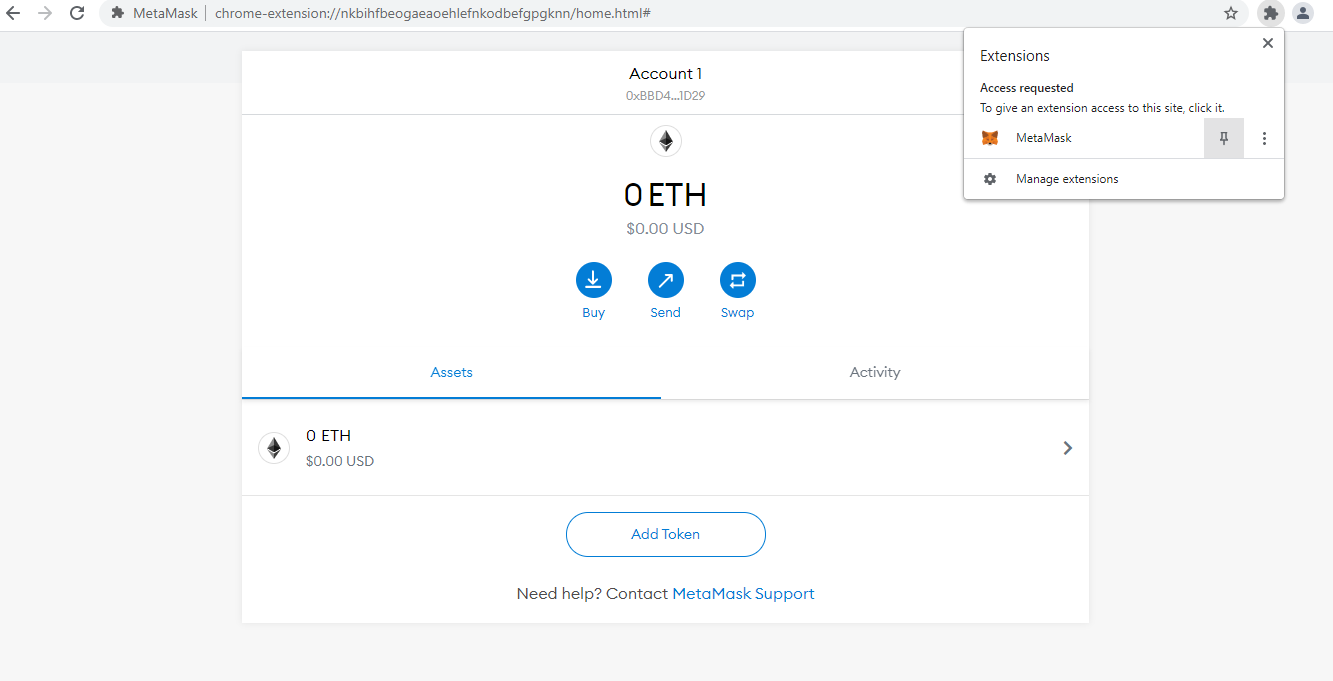
\includegraphics[scale=0.4]{metamask_new.png}}
  \caption{Creación de la wallet finalizada,  Fuente: captura de pantalla. }
  \label{img:metamask_new}
\end{figure}


\subsection{Desarrollo del Smart Contract}
Se utilizó Remix para  la edición del código fuente escrito en Solidity, este programa 
permite compilar el código para probarlo de manera local y también es una herramienta para publicarlo de manera online en otras Blockchain.
En este caso se publicó en Ropsten.

El código del smart contract se desarrolló siguiendo las definiciones de la sección \ref{s:system_design}, se encuentra en el anexo \ref{as:codigo_smart_contract}
En él se definieron los métodos ya mencionados y se agregaron reglas para que métodos en particulares puedan ser ejecutados solo por el propietario del smart contract y otros 
solo para los propietarios de las áreas.

El código desarrollado, cumple con los principios descriptos en otras secciones, 
y sigue algunas pautas de los estándares de certificados ya mencionados como BlockCerts y OpenCerts.
Algunas pautas son: almacenar información del emisor, almacenar el hash del documento, no relacionar datos
personales del propietario del documento digital.

 

% \begin{figure}[hbt!]
%   \centering
%   {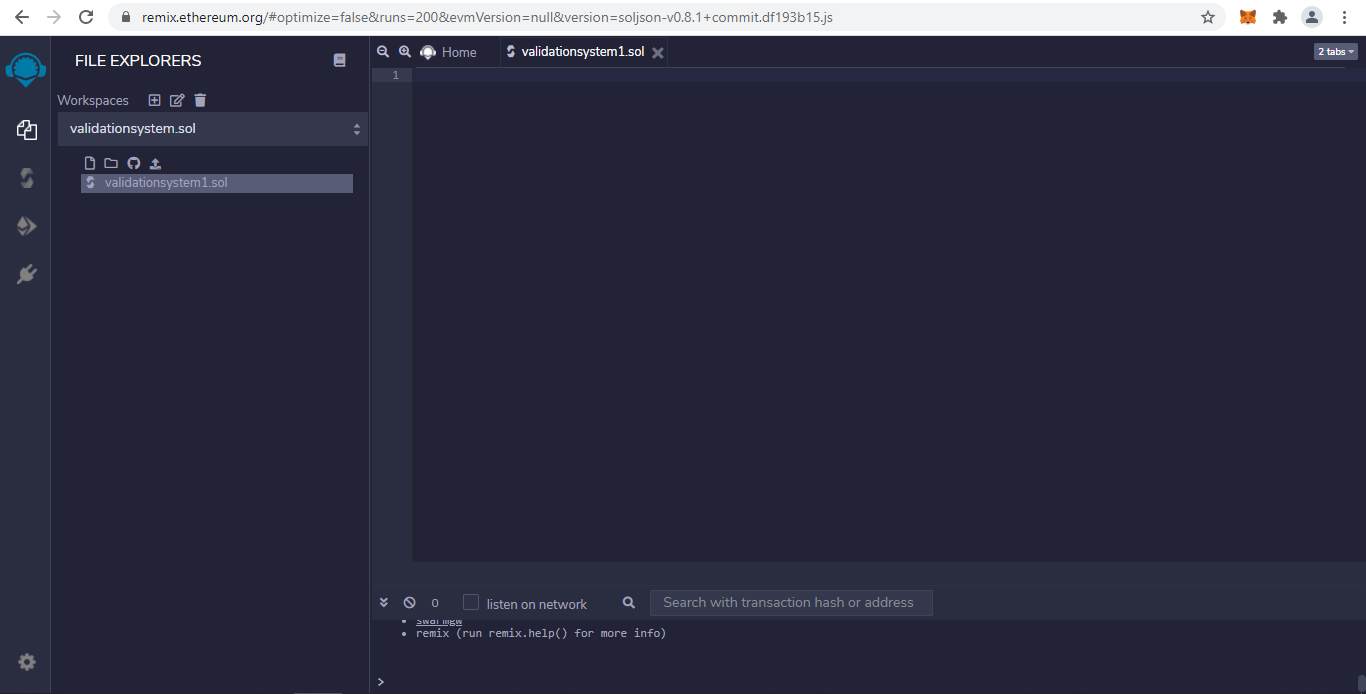
\includegraphics[scale=0.4]{validationSystem.png}}
%   \caption{Creando el smart contract con extensión “.sol”, Fuente: captura de pantalla. }
%   \label{img:valdationSystem}
% \end{figure}

Se desarrolla el código dentro del archivo “validationsystem.sol”, que tiene toda la lógica
del sistema con los comportamientos que se pueden realizar.
Una vez que el código está finalizado, hay que compilarlo, la figura   \ref{img:smart_contract_compile} muestra un ejemplo.
\begin{figure}[H]
  \centering
  {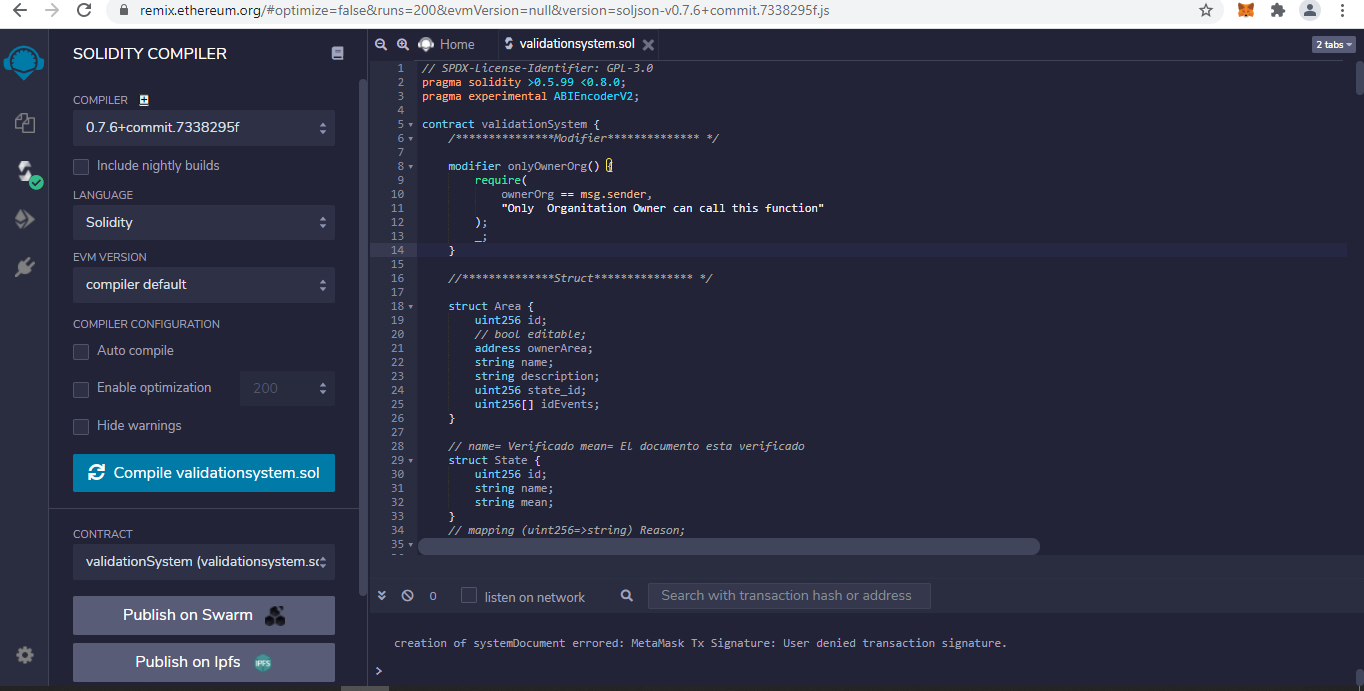
\includegraphics[scale=0.4]{smart_contract_compile.png}}
  \caption{Vista como compilar el contrato, Fuente: captura de pantalla. }
  \label{img:smart_contract_compile}
\end{figure}


Por otra parte es un requisito publicar el smart contract en alguna Blockchain, para ello hay que ejecutar Metamask y seleccionar la red de Ropsten 
como se muestra en la figura \ref{img:ropsten_selected}.
Luego es necesario conseguir la criptomoneda nativa de la Blockchain, 
para ello hay que acceder  a los sitios web denominados como \gls{faucet}, estos sitios 
web facilitan obtener las criptomonedas nativas. Para Ropsten se puede acceder al sitio web 
proporcionado por \href{https://faucet.metamask.io/}{Metamask}  o 
proporcionado por \href{https://faucet.ropsten.be/}{Ropsten} ambos sirven para obtener las criptomonedas para la red de prueba.  
\begin{figure}[H]
  \centering
  {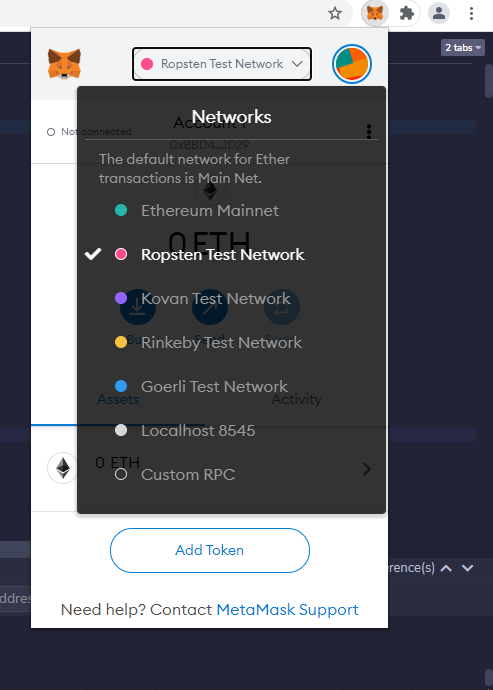
\includegraphics[scale=0.7]{Ropsten_seleteced.png}}
  \caption{Seleccionando la Red de Ropsten, Fuente: captura de pantalla. }
  \label{img:ropsten_selected}
\end{figure}

En este caso se utilizó el sitio web de la figura \ref{img:faucet_metamask} haciendo clic en el  botón verde,
suma 1 ETH a la cuenta.
\begin{figure}[H]
  \centering
  {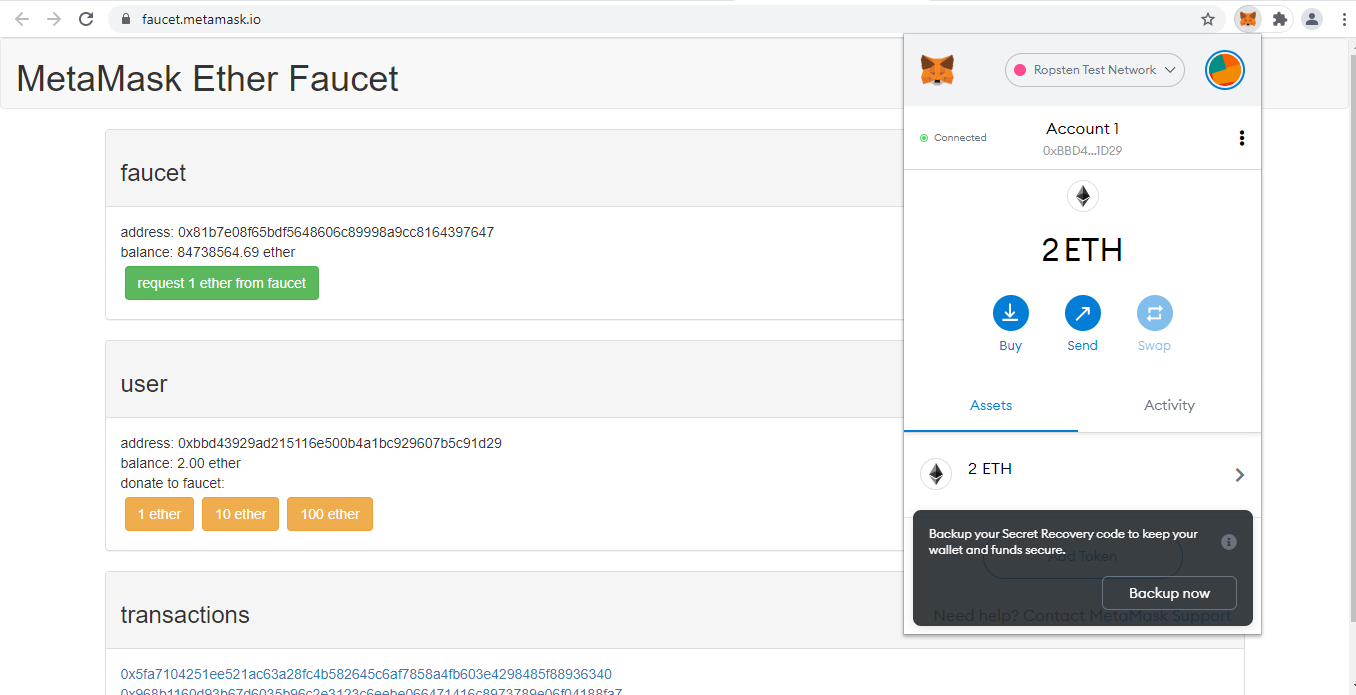
\includegraphics[scale=0.4]{FaucetMetamask.png}}
  \caption{Grifo de MetaMask, Fuente: captura de pantalla. }
  \label{img:faucet_metamask}
\end{figure}

A partir de ahora, se cuentan con todas las condiciones para publicar el código en la  Blockchain de Ropsten.
Para ello en el menú izquierdo de Remix  seleccionar la opción de  deploy, dentro de ella ir en la opción de “enviroment”  y seleccionar  “inject web3”, 
lo que abrirá Metamask requiriendo conectar la wallet con el sistema de Remix. Luego hacer clic al botón de color naranja (deploy) que se observa en la Figura \ref{img:remix_compile}

\begin{figure}[H]
  \centering
  {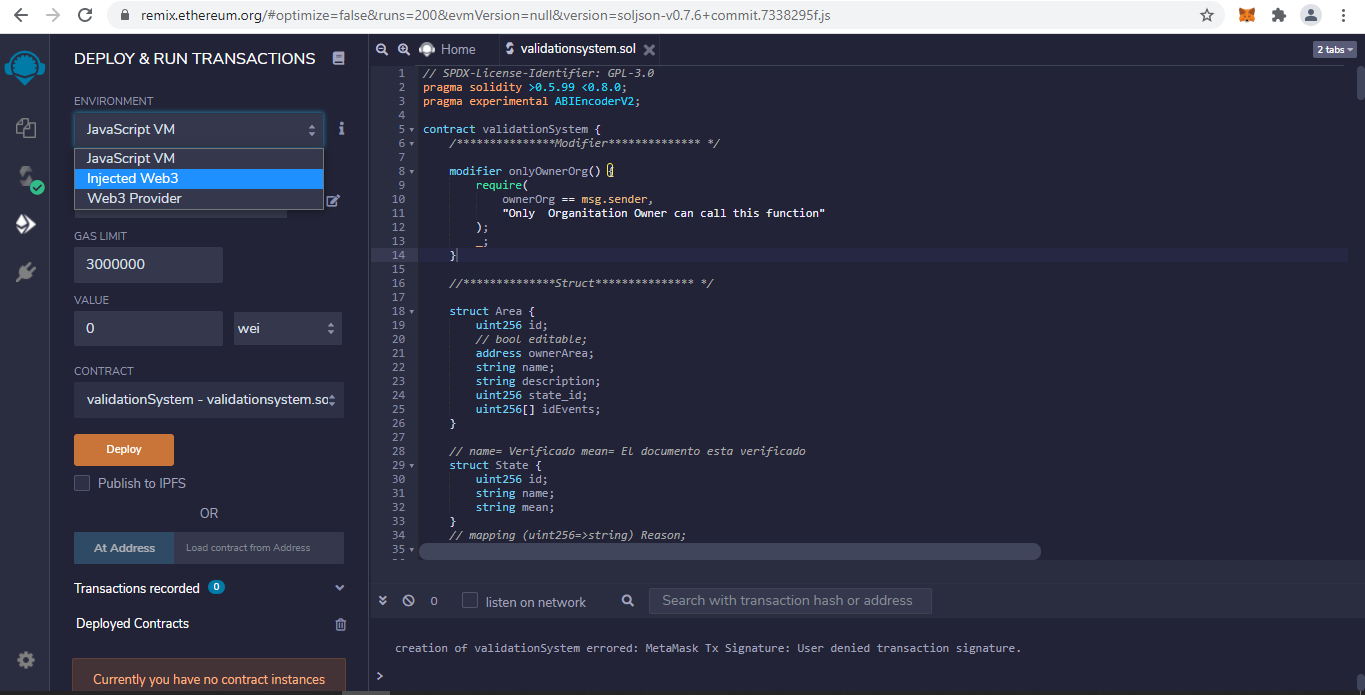
\includegraphics[scale=0.4]{remix_compile.png}}
  \caption{Menú deploy Remix, Fuente: captura de pantalla. }
  \label{img:remix_compile}
\end{figure}

\begin{figure}[H]
  \centering
  {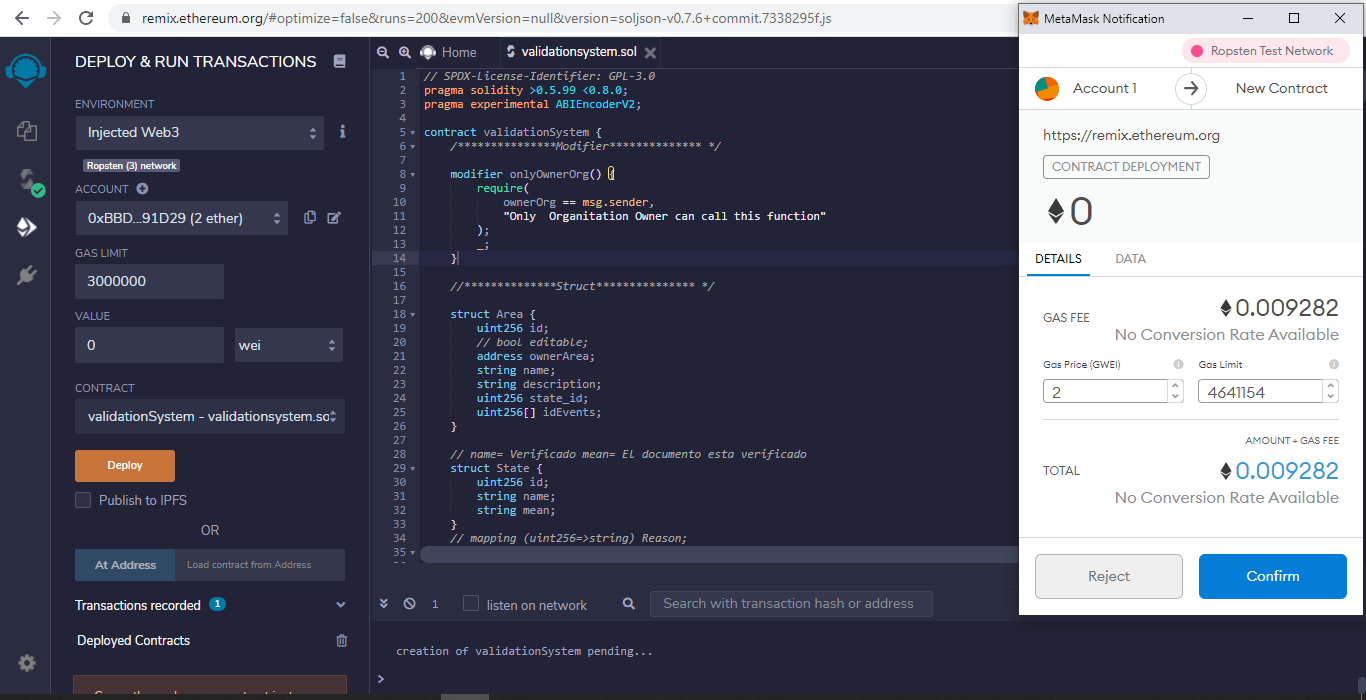
\includegraphics[scale=0.4]{remix_deploy.png}}
  \caption{Deploy Contrato Inteligente, Fuente: captura de pantalla. }
  \label{img:remix_deploy}
\end{figure}

Se abrirá una ventana de Metamask (Figura \ref{img:remix_deploy}), que pedirá la confirmación para gastar una cantidad de ETH, que es la criptomoneda
que se obtuvo mediante  la pagina web de grifo o faucet de Ropsten, la cual se utiliza para pagar las transacciones en la Blockchain.
Se confirma la transacción, y quedará en pendientes hasta ejecutarse, una vez finalizada el smart contract estará en la  Blockchain lista para
usarla.
En la figura \ref{img:metodos_contract_deploy} se muestran los métodos del contrato que se pueden ejecutar en la Blockchain, la interfaz
Remix también sirve para llamar a los diferentes métodos creados.
\begin{figure}[hbt!]
  \centering
  {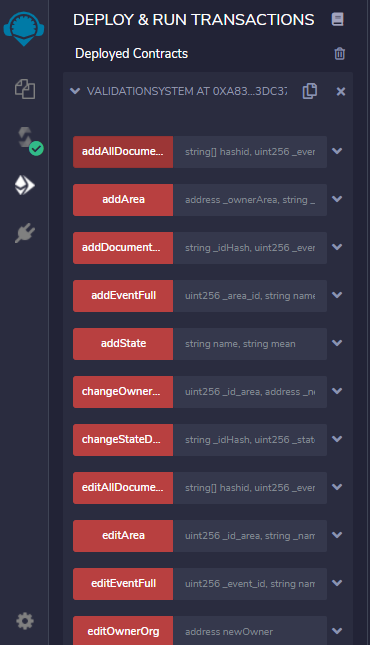
\includegraphics[scale=0.7]{Metodos_contract_deploy.png}}
  \caption{Contrato en la  Blockchain de Ropsten, Fuente: captura de pantalla. }
  \label{img:metodos_contract_deploy}
\end{figure}


\section{Desarrollo de la Interfaz de Usuario}
El desarrollo se realizó con el sistema operativo Windows 10 Home, pero
las herramientas pueden usarse en distribuciones de GNU/Linux.
Como primer paso se requiere instalar NODE JS desde su sitio oficial; también se utilizará Visual Studio Code como editor de texto.

Otro punto, es instalar  VUE JS CLI para facilitar la instalación de todos los paquetes y tener una estructura más organizada \cite[]{vue_cli_overview_2019},
para ello previamente se requiere instalar  NODE JS, en cmd o la consola de comandos del Visual 
Studio Code se ejecuta el comando “npm install -g @vue/cli”, para instalarlo de manera global,
en la figura \ref{img:INSTALL_VUE_CLI} se realiza utilizando Visual Studio Code.

\begin{figure}[H]
  \centering
  {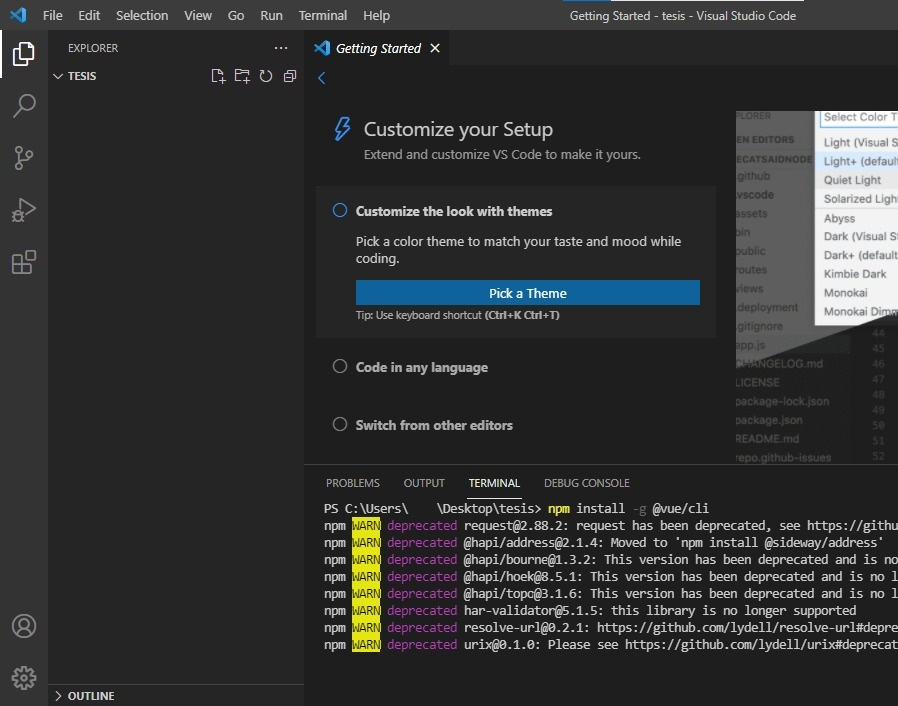
\includegraphics[scale=0.7]{INSTALL_VUE_CLI.jpeg}}
  \caption{Comando para instalar VUE CLI, Fuente: captura de pantalla. }
  \label{img:INSTALL_VUE_CLI}
\end{figure}

Luego en la consola de comandos hay que ubicarse en el directorio que se desea instalar el proyecto. Una vez hecho, ejecutar el comando 
“vue create nombre\_proyecto”, en este caso se usó “vue create validation\_system” esto abre unas opciones de configuraciones en consola, 
para el proyecto se utiliza router, vuex, babel; seleccionados estos ítems continuar con la instalación, en la figura \ref{img:vue_config} se muestra
las opciones necesarias para la creación del proyecto.
\newpage
\begin{figure}[H]
  \centering
  {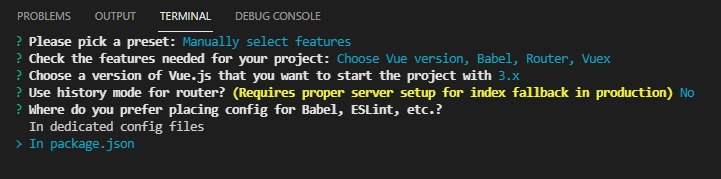
\includegraphics[scale=0.6]{VUE_Config.jpeg}}
  \caption{Configuración de proyecto, Fuente: captura de pantalla. }
  \label{img:vue_config}
\end{figure}

Como siguiente paso se debe ingresar dentro del directorio del proyecto creado en el cual se usarán dos librerías ya mencionadas ( web3 \cite[]{web3js_web3js_2016}, y sha256 \cite[]{satoh_asic-hardware-focused_2007}), 
también se usará un componente
que facilita la creación y carga de los select múltiples, mediante VUE. La instalación de estos se realiza con los comandos mostrados en la figura \ref{img:libreria}

\begin{figure}[hbt!]
  \centering
  {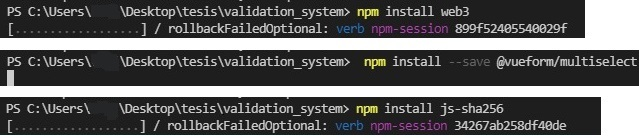
\includegraphics[scale=0.7]{librerias.jpeg}}
  \caption{Instalación de librerías y componente, Fuente: captura de pantalla. }
  \label{img:libreria}
\end{figure}

A partir de este punto comienza el desarrollo de la interfaz gráfica con las librerías y herramientas instaladas.

\subsection{Desarrollo de la Vista del Sistema}
Inicialmente, con la carpeta del proyecto generada se crean unos archivos extras, en este caso dentro de la ruta del proyecto “nombre\_proyecto/src/” se crea manualmente una carpeta con el nombre \/app donde
se almacenarán archivos que permitirán conectar con la Blockchain.

\begin{figure}[H]
  \centering
  {\includegraphics[scale=0.7]{ruta_archivo_Blockchain.png}}
  \caption{Archivos para conexión con la Blockchain, Fuente: captura de pantalla. }
  \label{img:ruta_archivo_Blockchain}
\end{figure}
El archivo abi.js define todos los métodos o funciones que se pueden usar en el smart contract creado, y  para eso 
hay que dirigirse a Remix, compilar nuevamente el código del smart contract y copiar el \gls{abi} creado. Por ejemplo, 
en la figura \ref{img:abi_copy} se resalta con un circulo rojo, el botón para copiar el \gls{abi}; este código se almacena 
dentro del archivo abi.js, ya que es utilizada para  las llamadas a los métodos.

\begin{figure}[H]
  \centering
  {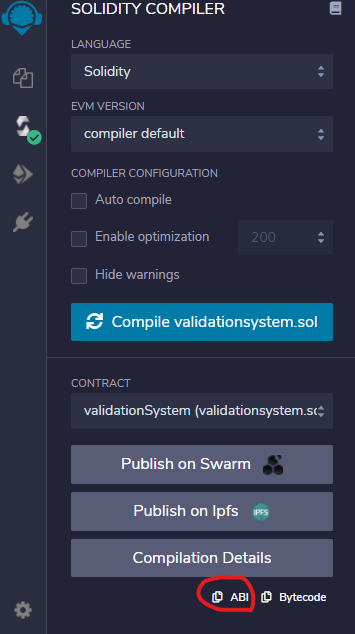
\includegraphics[scale=0.7]{ABI_Copy.png}}
  \caption{Copiar el ABI del código, Fuente: captura de pantalla. }
  \label{img:abi_copy}
\end{figure}

Posteriormente se crean una serie de archivos como app.js, document.js, parameters.js que contendrán la lógica para conectar la vista frontal con la Blockchain.
El último archivo parameters.js almacena la dirección del smart contract, la dirección se crea en el momento que se publicó el código con Remix,
la dirección generada es “\textbf{0x7006882779C21D8246 C82989F813237f78A781b1}”.


Las vistas desarrolladas  con VUE JS:
\begin{enumerate}
  \item \textit{Gestión de Área}: permite crear  Áreas, asignar un propietario mediante una dirección o clave pública, un nombre, descripción,
  a partir de él se pueden crear eventos.

  \begin{figure}[H]
    \centering
    {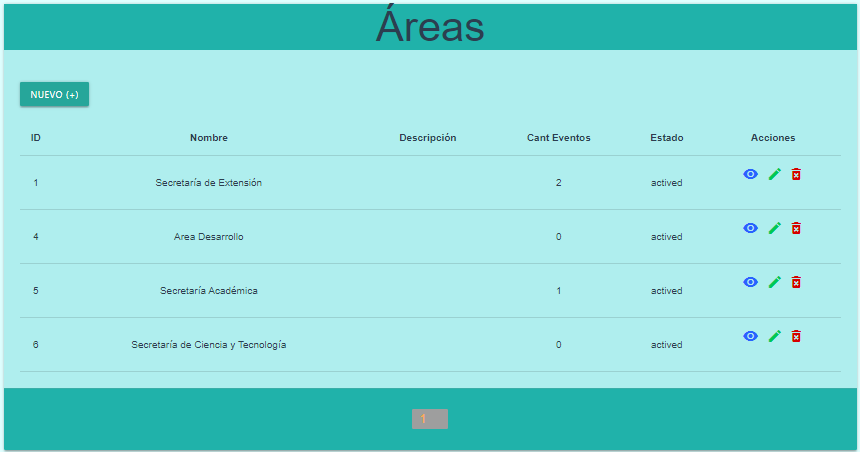
\includegraphics[scale=0.7]{Front_Area.png}}
    \caption{Vista de Áreas,  Fuente: captura de pantalla. }
    \label{img:front_area}
  \end{figure}

  \item \textit{Gestión de Evento}: se crean los Eventos encargados de generar los documentos, los datos para crear un evento son el nombre, 
  área relacionada, descripción, fecha de cuando inicio el evento, fecha cuando finaliza el evento y un estado. 
  Las fechas sirven para saber en que período se crearon los documentos, ya que cada documento está relacionado  a un evento.
  
  \begin{figure}[H]
    \centering
    {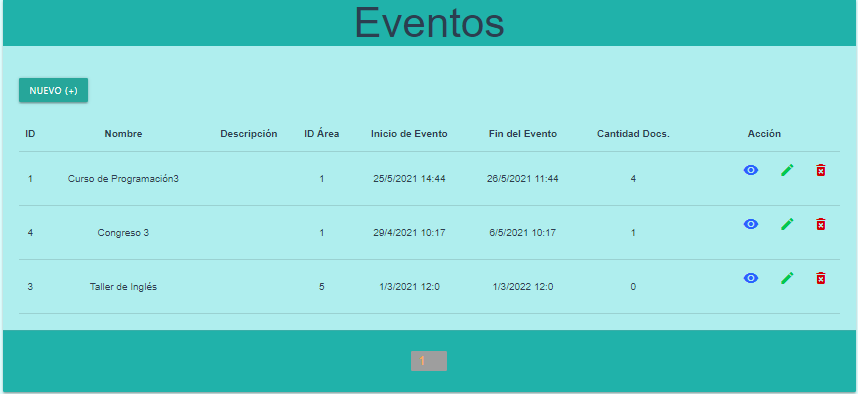
\includegraphics[scale=0.7]{Front_event.png}}
    \caption{Vista de Eventos,  Fuente: captura de pantalla. }
    \label{img:front_event}
  \end{figure}     
  
  \item \textit{Gestión de Documentos}: Se verifican o validan los documentos, si el usuario tiene el rol para crear documentos 
  también se utiliza como carga del mismo, si no tiene un rol solamente puede verificar si el documento fue registrada por la organización. 
  Un usuario propietario del área ve como se muestra en la figura \ref{img:front_document_owner}.

  \begin{figure}[H]
    \centering
    {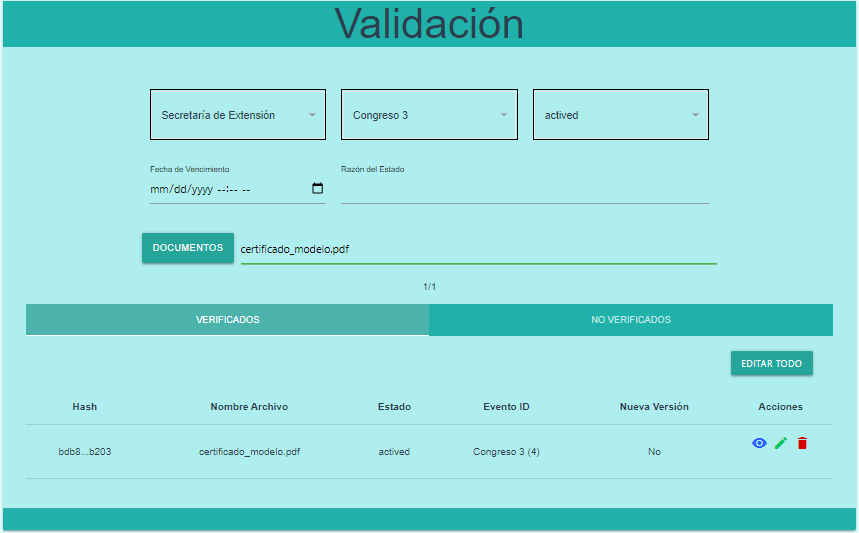
\includegraphics[scale=0.7]{Front_document_owner.png}}
    \caption{Vista de Documentos como propietario,  Fuente: captura de pantalla. }
    \label{img:front_document_owner}
  \end{figure}
  Y en el caso de una dirección pública que 
  no está registrada como propietario de un área o de la organización visualiza los documentos como en la figura \ref{img:front_document_public}.
  \begin{figure}[H]
    \centering
    {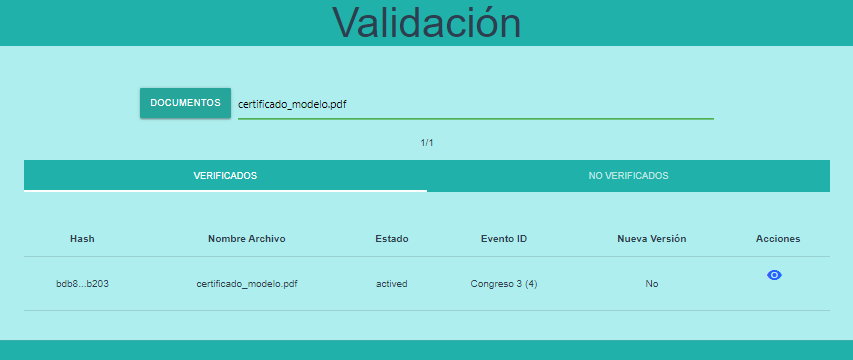
\includegraphics[scale=0.7]{front_document_public.png}}
    \caption{Vista de Documentos como usuario público,  Fuente: captura de pantalla. }
    \label{img:front_document_public}
  \end{figure}

  \item \textit{Gestión de Organización}: Mantiene los datos de la Organización, permite cambiar el nombre, cargar nuevos estados y cambiar al propietario de la organización, que 
  en este caso es el usuario que tiene permitido todas las acciones creadas.
  Los estados cargados por defecto son “deleted”, “actived”, “expired” y no pueden ser eliminados en el sistemas  ni modificados excepto “expired”. 

  \begin{figure}[H]
    \centering
    {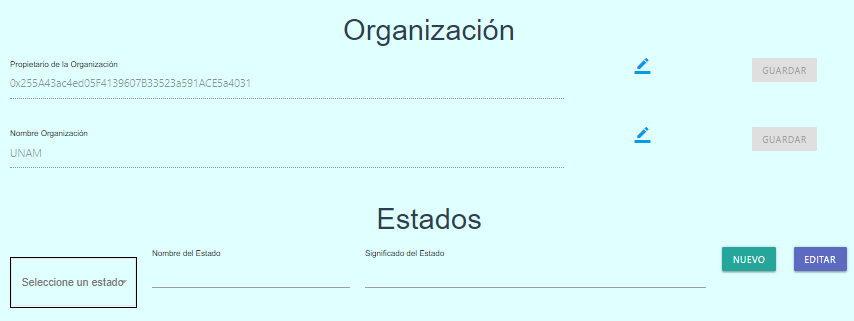
\includegraphics[scale=0.7]{front_org.png}}
    \caption{Vista de Organización,  Fuente: captura de pantalla. }
    \label{img:front_org}
  \end{figure}
\end{enumerate}


% El código completo del front end se encuentra en el repositorio de git \footnote{\url{https://github.com/agustinbritez/Sistema_Validacion.git}}.